\subsection{Conjunto de datos y Protocolo de Evaluación}
\label{subsection:evaluacion}


	El dataset utilizado para los experimentos es \textit{Chars74k} creado por T. E. Campos et al. en \cite{dCBV09}. El mismo consta de los siguientes tipos imágenes de caracteres: 
	\begin{itemize}
		\item \textbf{Escenas naturales:}
		
		Este conjunto de imágenes está dividido en 2 grupos: las imágenes buenas y las malas. A su vez, cada grupo contiene 62 subgrupos que representan a los caracteres alfanuméricos (en adelante clases) y que contienen varias imagenes representativas del carácter. En el presente trabajo, se hace uso de un subconjunto de todas estas imágenes creado por los autores de \textit{Chars74k}, llamado \textit{Chars74k-15}.
		
		\textit{Chars74k-15} consta de un conjunto de entrenamiento y uno de prueba, disjuntos entre si, con la misma estructura explicada para \textit{Chars74k} y contienen 15 imágenes por clase cada uno. Las imágenes de ambos conjuntos son una mezcla de las imágenes buenas y malas explicadas anteriormente. En los experimentos de este trabajo, se ajustaron las dimensiones de cada imágen a $48 \times 48$ píxeles. De esta forma, los descriptores de características de cada imágen tienen la misma dimensión. Cabe aclarar que el conjunto de evaluación descrito, se mantiene fijo durante todos los experimentos que se realizan en este trabajo. En la Figura \ref{fig: chars74k-reales} se muestra un ejemplo del conjunto de imágenes (buenas y malas) para el caracter ``K''.
		\begin{figure}[htbp]
			\centering
				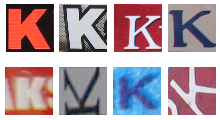
\includegraphics[scale=1]{img/img_buenas_malas.png}
				\caption[Chars74k reales]{Imágenes buenas (arriba) y malas (abajo) del carácter ``K''.}
			\label{fig: chars74k-reales}
		\end{figure}	
		
	\item \textbf{Sintéticos:}
	
	El conjunto de caracteres sintéticos, proviene de diversas fuentes de computadora. Este conjunto tiene una estructura similar a la anterior pero con algunas diferencias. La primera es que no se diferencian caracteres buenos de malos. La segunda es sobre la estructura en que estan representadas en el dataset \textit{Chars74k}. Cada clase contiene 1000 imágenes de caracteres de más de 40 fuentes diferentes en 3 estilos distintos (normal, itálica y negrita).
	
	En este trabajo, se utilizan estas imágenes para generar los datos sintéticos que se pueden observar en la Figura \ref{fig: chars74k-sint}. Como se detalló en la sección \ref{subsection:impl_propia}, para poder realizar esto se hacen uso de diferentes transformaciones fotométricas y geométricas. El objetivo, es intentar dar a la imagen el aspecto lo más parecido a una imagen natural.
	
		\begin{figure}[htbp]
			\centering
				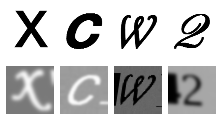
\includegraphics[scale=1]{img/synth_and_mod.png}
				\caption[Chars74k sinteticas]{Imágenes sintéticas. Arriba se pueden ver las imágenes sintéticas originales. Abajo se aprencia un conjunto de imágenes luego de aplicar las diferentes transformaciones.}
			\label{fig: chars74k-sint}
		\end{figure}	
		
		\item \textbf{Manuscritos:}
		
		Este conjunto esta compuesto más de 3400 caracteres escritos a mano. Tiene la misma estructura de grupos que los caracteres sintéticos y fueron extraidas utilizando una tablet-PC. Un ejemplo de este conjunto se puede observar en la Figura \ref{fig: chars74k-hand}. Cabe aclarar que en este trabajo no se utilizan este tipo de imágenes.
		
		\begin{figure}[htbp]
			\centering
			\subfloat{
				\fbox{ 
\includegraphics[scale=1]{img/hand/hand_1.png} }
			}
			\subfloat{
				\fbox{ 
\includegraphics[scale=1]{img/hand/hand_2.png} }
			}
			\subfloat{
				\fbox{ 
\includegraphics[scale=1]{img/hand/hand_3.png} }
			}
			\subfloat{
				\fbox{ 
\includegraphics[scale=1]{img/hand/hand_4.png} }
			}
			\caption[Chars74k manuscritas]{Imágenes de caracteres manuscritos.}
			\label{fig: chars74k-hand}
		\end{figure}
		
	\end{itemize}		
	
	Lo que calcula sobre el conjunto de evaluación (compuesto por imágenes naturales), es el grado de precisión del clasificador al haber entrenado al mismo con los conjuntos de entrenamiento explicados. Es decir, se buscar ver la cantidad de instancias correctamente clasificadas sobre el total de evaluadas.